
%(BEGIN_QUESTION)
% Copyright 2012, Tony R. Kuphaldt, released under the Creative Commons Attribution License (v 1.0)
% This means you may do almost anything with this work of mine, so long as you give me proper credit

Examine the primary and secondary connections on this three-phase transformer bank, and then determine the line voltage to the customer, assuming 7.2 kV line voltage on the distribution power lines.  The schematic diagram shown in the grey box is typical for each of the three transformers:

$$\includegraphics[width=15.5cm]{i02118x01.eps}$$

Assuming this is the last power pole on the line (i.e. the three 7.2 kV power lines dead-end at this transformer bank), calculate current through any one of those 7.2 kV lines if the line current to the customer is 49 amps.

\vfil 

\underbar{file i02118}
\eject
%(END_QUESTION)





%(BEGIN_ANSWER)

This is a graded question -- no answers or hints given!

%(END_ANSWER)





%(BEGIN_NOTES)

The transformer primary windings are connected in a Delta configuration, which means each primary winding receives the full 7.2 kV line voltage.  The secondary windings use one end and the center tap, each one effectively outputting 120 volts.  These are connected in a Wye configuration, making the secondary line voltage equal to 208 volts.

$$\includegraphics[width=15.5cm]{i02118x02.eps}$$

The effective winding ratio of each transformer is 7200:120, which is the same as 60:1.  This means each secondary winding carries 60 times more current than each primary winding.  If the customer's line current is 49 amps, and we know line current equals phase current in a Wye configuration (because each phase element is in series with a line conductor), then each 120 VAC secondary winding must be carrying 49 amps.  $1 \over 60$ of this current is 817 milliamps, which means each primary winding must be carrying this much.

Since the primary windings are connected to each other in a Delta configuration, their individual currents will combine to make a larger line current.  Thus, the amount of current through each 7.2 kV line will be:

$$\left( 49 \hbox{ A} \over 60 \right) \sqrt{3} = 1.415 \hbox{ A}$$

%INDEX% Electronics review: 3-phase electrical power 
%INDEX% Electronics review: AC transformer circuit
%INDEX% Process: AC power distribution system (transformer)

%(END_NOTES)


